\documentclass[a4paper,11pt,oneside]{Thesis}

\graphicspath{{Figures/}}

\usepackage[square,numbers,comma,sort&compress]{natbib}
\usepackage{longtable}
\usepackage{multirow}
\usepackage{tabularx}
\usepackage{makecell}
\usepackage{array}
\usepackage{enumitem}
\usepackage{float}
\usepackage{pdflscape}
\usepackage[table]{xcolor}
\usepackage{tikz}
\usetikzlibrary{arrows.meta,positioning,shapes.geometric,fit,calc}
\usepackage[ruled,vlined,linesnumbered]{algorithm2e}
\usepackage{microtype}
\usepackage{etoolbox}

\definecolor{dugreen}{RGB}{0,92,72}
\definecolor{dugold}{RGB}{193,145,44}
\definecolor{softgreen}{RGB}{226,241,235}
\definecolor{softblue}{RGB}{229,239,249}
\definecolor{softorange}{RGB}{252,237,216}
\definecolor{softgray}{RGB}{240,240,240}

\hypersetup{
  colorlinks=true,
  linkcolor=dugreen,
  citecolor=dugreen,
  urlcolor=blue,
  pdftitle={AI-Powered Business Analytics System for Performance Evaluation, Insight Extraction, and Strategy Optimization},
  pdfauthor={Md. Rakib Hossain and Shah Jamal Islam},
  pdfsubject={Initial Thesis Progress Report, February 2026 - February 2027},
  pdfkeywords={Bangladesh SMEs, business analytics, demand forecasting, customer segmentation, churn, explainable AI, B-SMART}
}

\newcommand{\system}{B-SMART}
\newcommand{\reportdate}{7 September 2026}
\newcommand{\projectperiod}{February 2026 - February 2027}
\newcommand{\cmark}{\cellcolor{softgreen}\textbf{C}}
\newcommand{\amark}{\cellcolor{softorange}\textbf{A}}
\newcommand{\pmark}{\cellcolor{softblue}\textbf{P}}
\newcommand{\na}{--}
\newcolumntype{Y}{>{\raggedright\arraybackslash}X}
\newcolumntype{C}[1]{>{\centering\arraybackslash}p{#1}}
\setlength{\emergencystretch}{2em}
\AtBeginEnvironment{thebibliography}{%
  \footnotesize
  \setstretch{1.0}%
  \renewcommand{\newblock}{\hspace{0.25em}}%
}

\begin{document}

\frontmatter
\begin{titlepage}
  \thispagestyle{empty}
  \enlargethispage{2cm}
  \begin{center}
    \vspace*{-1.4cm}
    {\Large\bfseries UNIVERSITY OF DHAKA\par}
    \vspace{0.20cm}
    {\large Department of Computer Science and Engineering\par}
    \vspace{0.25cm}

    
\includegraphics[width=1.15in]{logo.pdf}\par
    \vspace{0.25cm}

    {\Large\bfseries AI-Powered Business Analytics System for\\[0.15cm]
    Performance Evaluation, Insight Extraction, and\\[0.15cm]
    Strategy Optimization\par}
    \vspace{0.30cm}
    {\large\bfseries Thesis Progress Report\par}
    \vspace{0.15cm}
    {\normalsize Project Period: \projectperiod\par}
    {\normalsize Status Date: \reportdate\par}

    \vspace{0.25cm}
    {\normalsize Submitted by\par}
    \vspace{0.15cm}
    \begin{tabular}{c}
      \textbf{Md. Rakib Hossain} \\
      Roll: 88 \quad Registration No.: 2020315665 \\[0.20cm]
      \textbf{Shah Jamal Islam} \\
      Roll: 81 \quad Registration No.: 2020915641
    \end{tabular}

    \vspace{0.25cm}
    {\normalsize Supervised by\par}
    \vspace{0.12cm}
    {\large\bfseries Dr. Saifuddin Md. Tareeq\par}
    {\normalsize Professor\par}
    {\normalsize Department of Computer Science and Engineering\par}
    {\normalsize University of Dhaka\par}

    \vspace{0.15cm}
    {\normalsize CSE 4114 - Project Work\par}
    {\normalsize 4th Year 1st Semester Examination 2025 \quad September 2026\par}
  \end{center}
\end{titlepage}
\cleardoublepage

\setstretch{1.15}
\pagestyle{fancy}
\fancyhead{}
\rhead{\thepage}

\Declaration{
  This initial report presents the foundation of the thesis project entitled
\emph{AI-Powered Business Analytics System for Performance Evaluation,
Insight Extraction, and Strategy Optimization}. We declare that the background
study, problem formulation and proposed methodology presented here are the work
of the authors under the supervision of Dr. Saifuddin Md. Tareeq. Ideas,
methods, datasets and findings originating from prior work are cited. The
implementation, experimental results and conclusions are intentionally reserved
for later stages of the thesis. This report is current to \reportdate; the
project remains in progress until February 2027.

\vspace{1.2cm}
\begin{tabularx}{\textwidth}{X X}
  \rule{5.2cm}{0.4pt} & \rule{5.2cm}{0.4pt} \\
  Md. Rakib Hossain & Shah Jamal Islam \\
  Candidate & Candidate \\
  \\[1.0cm]
  \rule{5.2cm}{0.4pt} & \\
  Dr. Saifuddin Md. Tareeq & \\
  Supervisor &
\end{tabularx}

}
\clearpage

\addtotoc{Abstract}
\begin{center}
  {\huge\textit{Abstract}\par}
\end{center}
% Intentionally left blank for the initial progress submission.
% The abstract will be completed in the final thesis.

\clearpage

\acknowledgements{
  We express our sincere gratitude to our supervisor, Dr. Saifuddin Md. Tareeq,
Professor, Department of Computer Science and Engineering, University of
Dhaka, for defining the academic direction of this work and for emphasizing
clear problem formulation, literature coverage, sequential methodology,
scalability evaluation and honest reporting. We also thank the faculty and
staff of the department for the facilities and guidance that support this
project. Finally, we acknowledge the maintainers of the public datasets and
open-source software used for reproducible method validation. Responsibility
for the implementation, analysis and any remaining errors belongs to the
authors.

}
\clearpage

\lhead{\emph{Contents}}
\setcounter{tocdepth}{2}
\tableofcontents

\lhead{\emph{List of Figures}}
\listoffigures

\lhead{\emph{List of Tables}}
\listoftables


\mainmatter
\pagestyle{fancy}
\fancyhead{}
\rhead{\thepage}
\lhead{\fancyplain{}{\rightmark}}
\setstretch{1.14}
\renewcommand{\sectionmark}[1]{\markright{\thesection\ #1}}

\chapter{Introduction}
\label{chapter_introduction}

\section{Context and Motivation}

Business intelligence and analytics organize operational data so that decision
makers can describe performance, anticipate future conditions and choose an
appropriate response \cite{chen2012business}. For an inventory-based small or
medium enterprise (SME), this progression begins with familiar records: invoice
lines, product movements, purchase receipts, expenses, payments and customer
visits. These records can explain revenue and stock position, but their value is
limited when they remain divided among paper ledgers, spreadsheets and separate
applications. The owner may know that sales declined last month without knowing
which products, customers or operating conditions caused the decline, whether
the pattern is likely to continue, or which affordable action should be taken.

The decision is more demanding than producing a dashboard. Before Ramadan or
Eid, for example, a retailer must estimate demand early enough to order from a
supplier. Ordering too little creates stock-outs and forgone sales; ordering too
much immobilizes working capital and may create obsolete stock. At the same
time, a previously valuable customer may be becoming inactive, a product may
appear profitable only because costs were recorded incompletely, or a promotion
may increase volume without increasing contribution. These questions draw on
the same operational history but require different analytical tasks and a
common decision context.

Retail forecasting research identifies hierarchy, intermittency, promotions,
new products, changing assortment and the organizational use of forecasts as
central practical concerns \cite{fildes2022retail}. Evidence from large forecast
competitions also cautions against assuming that a more complex algorithm is
automatically more accurate: combinations, statistical methods and carefully
constructed baselines remain competitive across many series
\cite{makridakis2022m5}. The relevant research problem is
therefore not to attach a fashionable model to a sales file. It is to construct
a defensible path from business events to out-of-time predictions and then from
predictions to feasible, explainable actions.

\section{Bangladesh SME Context}

The intended setting is an inventory-holding retail SME in Bangladesh. This
scope is narrower than the approved thesis title, but it makes the business
entities, prediction units and decisions testable. Bangladesh-specific studies
show that ICT adoption in SMEs is shaped by perceived benefit, management and
government support, cost, complexity and the surrounding organizational and
technological conditions \cite{hoque2016ict,shahadat2023digital}. Research on
mobile financial services further shows that users value accessibility,
mobility, self-control and other affordances embedded in everyday practice
\cite{hazra2021mfs}. These findings imply that local payment channels,
low-friction data entry and owner-readable explanations are design requirements,
not optional presentation details.

This study uses a functional definition of its population rather than relying
on a regulatory size threshold that may change. A target business holds stock,
records sales and purchases, makes branch- or product-level decisions, and has
limited specialist analytics capacity. The unit of analysis may be a business,
branch, stock-keeping unit (SKU), customer or historical customer snapshot,
depending on the research question. Conclusions will be restricted to the
participating firms and the evidence actually collected.

\section{Problem Statement}

The central problem is the absence of a trustworthy and usable connection among
three activities: recording SME operations, extracting predictive insight and
selecting a feasible business action. A transaction system can preserve orders
and stock but still provide no forecast. A standalone model can report an
accuracy score but still be unusable because its features would not exist at the
decision time, its test data leaked information from training, or its output is
not linked to budget, stock, lead time and customer consent. A recommendation
can be technically valid yet operationally impossible.

The problem is decomposed into four linked gaps:

\begin{enumerate}[label=G\arabic*.]
  \item \textbf{Data foundation gap.} Sales, inventory, purchases, expenses,
  customers and payments need a consistent schema, timestamps, provenance and
  organization boundaries before they can support comparable analytics.
  \item \textbf{Prediction-validity gap.} Demand and customer-risk models must
  use historical snapshots, chronological or entity-safe splits, training-only
  transformations, strong baselines and metrics appropriate to sparse or
  imbalanced outcomes. Leakage can otherwise create persuasive but invalid
  performance \cite{kaufman2012leakage}.
  \item \textbf{Decision gap.} A forecast or risk probability does not specify
  what to order, whom to contact or whether the action is affordable. Prediction
  must be connected to costs, constraints and uncertainty; this is the
  transition from predictive to prescriptive analytics
  \cite{bertsimas2020prescriptive}.
  \item \textbf{Adoption and accountability gap.} An SME owner needs a concise
  reason, confidence indication and traceable source for a suggestion. Feature
  attribution can describe model behavior, but it neither proves causality nor
  replaces human judgment \cite{lundberg2017shap,miller2019explanation}.
\end{enumerate}

Accordingly, this thesis asks how an integrated, Bangladesh-aware framework can
transform auditable retail records into leakage-controlled forecasts and
customer insights, and then rank actions that respect the operating constraints
of an SME. The work does not presume that machine learning will defeat every
baseline. Discovering that a simple rule is more reliable or economical for a
particular task is a valid outcome.

\section{Research Aim and Objectives}

\subsection{General Objective}

The general objective is to design and evaluate an AI-powered business
analytics framework that enables Bangladeshi retail SMEs to monitor performance,
extract reliable and explainable insights, and prioritize feasible strategies.

\subsection{Specific Objectives}

The study will:

\begin{enumerate}[label=O\arabic*.]
  \item define an auditable canonical data model for sales, products, stock,
  purchases, returns, customers, suppliers, payments and expenses;
  \item construct reproducible, time-indexed preprocessing and feature pipelines
  for performance analysis, SKU demand, customer inactivity and segmentation;
  \item compare simple, statistical and machine-learning approaches under
  chronological or entity-safe validation, using both predictive and
  decision-oriented measures;
  \item quantify uncertainty and provide global and case-level supporting
  factors without presenting association as causation;
  \item formulate a constraint-aware mechanism for reorder, retention and
  operational action ranking; and
  \item evaluate technical accuracy, robustness, scalability, usability and
  potential business value on clearly separated evidence tiers, culminating in
  consenting Bangladeshi SME data.
\end{enumerate}

\section{Initial Solution Concept}

The proposed solution is \system{}: the Bangladesh SME Monitoring, Analytics,
Recommendation and Tracking framework. It is an end-to-end decision-support
process rather than a new base classifier. Business events enter a governed
operational layer; validated events are transformed into time-frozen analytical
views; candidate models generate forecasts, risks and segment profiles; and a
strategy layer removes infeasible actions before ranking the remainder. Each
displayed action carries its data cutoff, model or baseline source, uncertainty
and supporting factors. Owner response and later outcome are retained for
evaluation and monitoring.

Three analytical outputs match the approved title. \emph{Performance
evaluation} summarizes revenue, margin, stock movement and customer behavior
from reconciled records. \emph{Insight extraction} estimates future demand and
customer inactivity and identifies meaningful behavioral groups.
\emph{Strategy optimization} converts those estimates into candidates such as a
reorder quantity or retention priority, subject to cash, storage, lead time,
minimum order quantity, current stock and contact consent. Chapter
\ref{chapter_methodology} defines these components formally.

\section{Research Questions}

The thesis is guided by four questions:

\begin{description}[style=nextline,leftmargin=0pt]
  \item[RQ1.] Do calendar, price, promotion and market-context features improve
  out-of-time branch--SKU demand forecasts over seasonal and statistical
  baselines in the target SME setting?
  \item[RQ2.] How accurately and reliably can a historical customer snapshot
  identify no repeat purchase during a fixed future horizon?
  \item[RQ3.] Under the same demand and operating constraints, does a
  forecast-driven reorder policy reduce stock-out and holding cost relative to
  the participating business's current policy?
  \item[RQ4.] Do concise Bangla action explanations improve owner task
  completion, confidence and perceived usability without creating excessive
  decision time?
\end{description}

\section{Scope and Boundaries}

The research covers retail and inventory-based SMEs, structured operational
data, descriptive indicators, demand forecasting, customer inactivity,
behavioral segmentation, explanation and two strategy families: replenishment
and consent-aware customer retention. The initial geographical context is
Bangladesh; an external dataset may test method portability but cannot establish
Bangladeshi business behavior. Public price data may supply market context but
cannot substitute for invoice-level evidence.

The study excludes manufacturing scheduling, credit scoring, employee
surveillance, fully autonomous price changes and unrestricted customer
profiling. It does not claim causal effects from observational feature
attributions. It will not treat generated data as field evidence, combine
synthetic and real observations in a reported real-world score, or generalize
from one retailer to all SMEs. Implementation detail, experimental results and
final conclusions are deliberately reserved for Chapters
\ref{chapter_implementation}--\ref{chapter_conclusion}.

\section{Expected Contributions and Significance}

The expected research contribution is the evaluated integration of established
methods under constraints that matter to small retailers. Specifically, the
work is expected to provide: (i) a traceable operational-to-analytical data
design; (ii) reusable historical-snapshot protocols that prevent common forms
of leakage; (iii) a Bangladesh-aware comparison of forecasting and customer
analytics baselines; (iv) a transparent bridge from prediction to constrained
action; and (v) evidence about whether owners can correctly interpret and use
the resulting recommendations.

The practical significance is equally bounded. The proposed system is intended
to help an owner see the evidence behind a decision, compare a recommendation
with a familiar rule and retain authority over the final action. It is not
intended to remove the owner from the decision or to label a statistically
accurate output as profitable before business impact is measured.

\section{Anticipated Challenges}

The most consequential dependency is suitable primary data. The intended joint
history of invoice lines, stock, products, prices and customers is difficult to
obtain from a public Bangladesh source, and partner data may contain missing
identifiers, changing SKU codes or incomplete cost records. Technical risks
include intermittent demand, short histories, new products, stock-out censoring,
class imbalance and drift. Scientific risks include target leakage, optimistic
model selection, incompatible dataset comparisons and conclusions based on one
firm. Human risks include time pressure, varied digital skill, low trust and
over-trust in confident-looking explanations. The methodology assigns a
specific prevention or evaluation step to each of these risks.

\section{Organization of the Report}

Chapter~\ref{chapter_backStudy} develops the technical and contextual
background, reviews the verified literature and identifies the research gap.
Chapter~\ref{chapter_methodology} presents the research design, data protocol,
formal tasks, proposed framework, evaluation plan and two-semester timeline.
The Implementation and Experimental Results chapters remain named placeholders
in this initial report. The Conclusions chapter synthesizes only what can be
established from the present background study and proposed methodology; final
outcome conclusions require the later empirical evidence.

\cleardoublepage
\chapter{Background Study and Related Work}
\label{chapter_backStudy}

\section{Background Study}

\subsection{Business Intelligence and the Decision Continuum}

Business intelligence (BI) combines data, infrastructure, analytical methods
and organizational practice to improve decisions. Chen, Chiang and Storey trace
its development from structured enterprise reporting toward web, mobile and
sensor-rich analytics \cite{chen2012business}. This thesis adopts a three-stage
decision continuum. \emph{Descriptive analytics} establishes what happened and
where; \emph{predictive analytics} estimates what may happen next; and
\emph{prescriptive analytics} compares feasible responses. The stages are
dependent: an action recommendation is only as credible as the prediction that
supports it, and a prediction is only as credible as the operational data from
which it was derived.

Operational and analytical workloads also have different integrity needs. A
sale requires a consistent stock and payment update, whereas a model requires a
historical feature view whose values do not change after evaluation. The
proposed framework therefore separates the transaction record from versioned
analytical snapshots. It retains the relationship between them through source
identifiers, timestamps and transformation metadata.

\subsection{SME Digitalization in Bangladesh}

Technology adoption is not determined by model accuracy alone. A mixed-method
case study of rural Bangladeshi SMEs identifies awareness of benefits,
government support, top-management support and financial support as important
ICT-adoption determinants \cite{hoque2016ict}. A later survey of 535 SME
managers combines the technology--organization--environment framework with
diffusion-of-innovation constructs; relative advantage, complexity, perceived
cost, management factors, competitive pressure and government support are among
the significant determinants reported \cite{shahadat2023digital}. These studies
justify attention to cost, workflow fit and organizational readiness, although
neither evaluates a retail prediction system.

Mobile financial services are part of this operating context. Interview-based
research in Bangladesh identifies accessibility, spatial and temporal mobility,
self-control and related affordances in everyday MFS use
\cite{hazra2021mfs}. Consequently, the proposed data model treats payment mode
and settlement status as ordinary business fields. The research does not infer
that a particular provider causes better performance; it asks whether locally
recognizable records and explanations make the analytical workflow more usable.

\subsection{Performance Evaluation and Data Foundations}

Performance evaluation begins with well-defined measures. Revenue, gross
margin, average order value, stock turnover, return rate and customer-repeat
rate must each specify a time window, aggregation level and treatment of
cancellations, refunds and missing costs. A dashboard value without these
definitions can disagree with the accounting record or compare unlike periods.
The canonical layer therefore preserves invoice lines and stock movements while
deriving analytical measures in documented views.

Data provenance answers where a record came from, when it was received and how
it was transformed. For primary SME data, provenance must be joined with
organization isolation and pseudonymous customer identifiers. For public data,
the license, original context and permissible inference must be recorded. A
foreign transaction dataset can test whether code handles real invoices but
cannot establish Bangladesh-specific customer behavior.

\subsection{Customer Analytics: RFM, CLV and Segmentation}

RFM summarizes \emph{recency}, \emph{frequency} and \emph{monetary value} from
a customer's transaction history. These features are inexpensive to derive and
retain a clear behavioral interpretation. Fader, Hardie and Lee connect RFM to
customer lifetime value (CLV) through Pareto/NBD and gamma--gamma components and
show how different histories can have similar expected value
\cite{fader2005rfm}. CLV is useful as an outcome or planning quantity, but a
field used to define a segment cannot also be admitted as an independent
predictor of that same segment.

Unsupervised segmentation asks whether coherent behavioral groups emerge
without an existing label. For K-Means, the objective is

\begin{equation}
  \underset{\{C_k,\mu_k\}_{k=1}^{K}}{\operatorname{minimize}}
  \sum_{k=1}^{K}\sum_{x_i\in C_k}\lVert x_i-\mu_k\rVert_2^2.
  \label{eq:kmeans}
\end{equation}

Because the procedure returns clusters even when the data form a continuum,
cluster number and interpretation require validation. The silhouette
coefficient compares within-cluster cohesion with separation from the nearest
other cluster \cite{rousseeuw1987silhouettes}. Stability under resampling and
business usefulness are separate tests; an attractive label such as ``loyal''
does not establish that a cluster is statistically stable or actionable.

\subsection{Retail Demand Forecasting}

A demand forecast estimates the units required for a defined product, location
and future horizon. Retail series may be affected by price, promotion,
stock-outs, festivals, assortment changes and aggregation across products or
branches. Fildes, Ma and Kolassa emphasize that retail forecasting practice
cannot be reduced to a single algorithm because data hierarchy, operational
process and forecast use matter alongside statistical accuracy
\cite{fildes2022retail}.

Intermittent SKU demand contains many zero periods separated by nonzero demand.
Croston's method separately smooths nonzero size and the interval between
demands \cite{croston1972intermittent}; Syntetos and Boylan analyze bias and
accuracy in intermittent-demand estimates \cite{syntetos2005intermittent}.
These works motivate an intermittent-demand baseline instead of forcing every
SKU through a dense-series model. At the same time, forecasts must reconcile
across product, category, branch and business totals. Optimal-combination
reconciliation offers a principled way to produce coherent hierarchical
forecasts \cite{hyndman2011hierarchical}.

Model complexity should follow the evidence. ARIMA-family models represent
serial dependence after transformation; tree ensembles can learn nonlinear
effects from lagged, calendar and price variables; LSTM networks use gated
memory for sequential dependence \cite{hochreiter1997lstm}. Random Forest and
XGBoost provide strong tabular comparators \cite{breiman2001rf,chen2016xgboost}.
However, forecast competitions show that statistical, combined and hybrid
approaches remain highly competitive across large collections
\cite{makridakis2018m4,makridakis2022m5}. A seasonal-naive forecast is therefore
a required benchmark, not a ceremonial baseline.

Forecast accuracy and inventory usefulness are related but not identical.
Hyndman and Koehler demonstrate defects in common percentage errors and propose
MASE for scale-free comparison \cite{hyndman2006accuracy}. Syntetos and
colleagues connect forecast selection with stock-control performance in a
wholesaling study \cite{syntetos2010stock}. The methodology accordingly reports
point error, uncertainty and simulated stock-out/holding cost rather than
selecting a method from one convenient metric.

\subsection{Customer Inactivity, Class Imbalance and Calibration}

In a subscription service, churn may be an observed cancellation. In
non-contractual retail it must be defined at a cutoff $t$: no repeat purchase
during a fixed interval $(t,t+H]$. Every feature must be known by $t$, and the
future label window must not contaminate training or validation. This definition
turns an ambiguous business word into a reproducible prediction task.

The positive class may be rare or change across businesses. Burez and Van den
Poel show that sampling and cost-sensitive treatments affect churn modelling
under class imbalance \cite{burez2009imbalance}. Saito and Rehmsmeier explain
why precision--recall analysis is more revealing than ROC analysis for
imbalanced binary tasks \cite{saito2015pr}. Verbeke and colleagues further show
that the best discriminating churn model need not be the most profitable when
contact cost and benefit are considered \cite{verbeke2012profit}.

Ranking is not enough when the output is used in a decision calculation. A
probability of $0.7$ should correspond, approximately, to the event frequency
among comparable cases. Niculescu-Mizil and Caruana compare probability
estimates and post-hoc calibration methods for supervised learners
\cite{niculescu2005calibration}. The proposed framework therefore reports Brier
score and calibration in addition to PR-AUC, ROC-AUC and top-fraction lift.

\subsection{Leakage, Explainability and Change Over Time}

Data leakage arises when training has access to information that would not
legitimately exist at prediction time. It may enter through a target-derived
field, a post-outcome variable, repeated customers in both sides of a split or a
transform fitted before the split \cite{kaufman2012leakage}. Leakage control is
therefore a property of the entire data pipeline, not a model option. A clear
prediction time, feature availability table and split policy precede training.

SHAP represents a prediction as additive feature contributions relative to a
reference value \cite{lundberg2017shap}; efficient tree-specific methods support
local and global inspection \cite{lundberg2020trees}. Such an attribution
describes how a fitted model used encoded features. Miller's synthesis of social
science research emphasizes that useful explanations are selective, contextual
and often contrastive \cite{miller2019explanation}. Thus a recommendation card
should answer ``why this action now?'' in a small number of decision-relevant
factors, while preserving access to fuller evidence and avoiding causal wording.

Business conditions also change. Concept drift occurs when the relationship
between predictors and outcomes changes over time; Gama and colleagues organize
adaptation methods and evaluation strategies for this setting
\cite{gama2014drift}. Retail monitoring must distinguish data-quality failure,
input-distribution shift and performance decay. A retraining schedule alone is
not evidence that a model remains valid.

\subsection{From Prediction to Constrained Action}

Prescriptive analytics uses predictions within an explicit decision problem.
Bertsimas and Kallus formulate data-driven prescriptions in which auxiliary
observations inform conditional stochastic optimization
\cite{bertsimas2020prescriptive}. The present thesis adopts the underlying
principle---evaluate actions by expected benefit, cost and constraints---without
claiming to reproduce that paper's asymptotic method. Reorder and retention are
kept as separate action families because their outcomes, costs, permissions and
uncertainties differ.

The complete framework is an information-system artifact as well as an
analytical study. Design-science research builds and evaluates artifacts in
relation to a relevant problem and a knowledge base \cite{hevner2004design}.
This supports an evaluation plan that includes predictive validity, software
behavior, owner usability and decision consequences instead of reporting model
accuracy as the sole measure of success.

\section{Literature-Review Procedure}
\label{sec:literature_review}

The present review is a structured background study, not a claim of an
exhaustive systematic review. Sources were selected for direct relevance to one
of six themes: Bangladesh SME digitalization, BI and design science, customer
analytics, retail demand/inventory, churn and evaluation integrity, and
explainable or prescriptive analytics. Searches used combinations of terms such
as \emph{Bangladesh SME ICT adoption}, \emph{retail demand forecasting},
\emph{intermittent demand}, \emph{RFM customer segmentation}, \emph{churn
profit}, \emph{data leakage}, \emph{probability calibration}, \emph{concept
drift} and \emph{prescriptive analytics}.

Peer-reviewed journal or conference work was preferred. A source was retained
when it defined a required concept, supplied a method or evaluation principle,
or provided Bangladesh-specific evidence. Metadata for every DOI-bearing entry
was checked against Crossref, and dataset records were checked against DataCite
or the official repository. Specific numerical claims were included only when
supported by the paper metadata, abstract or full record available to the
authors. The core set contains 33 scholarly works; candidate datasets are listed
separately in Chapter~\ref{chapter_methodology}.

\section{Thematic Synthesis of Prior Work}

\subsection{Business and Bangladesh Evidence}

The BI literature supplies the descriptive--predictive--prescriptive frame
\cite{chen2012business}, while design science supplies an artifact-oriented
research logic \cite{hevner2004design}. Bangladesh studies explain why
organizational support, perceived value, cost, complexity and actual local use
should influence the proposed design \cite{hoque2016ict,shahadat2023digital,
hazra2021mfs}. Their limitation for the present problem is not quality but unit
of analysis: adoption surveys and interviews do not provide invoice-level
evidence for demand, inactivity or inventory decisions.

\subsection{Customer Evidence}

Ngai, Xiu and Chau classify 87 CRM data-mining studies selected from a much
larger screened body and show the breadth of classification, association and
retention applications \cite{ngai2009crm}. Fader et al. provide a probabilistic
link between transaction history and future value \cite{fader2005rfm}; Kim et
al. connect customer value with segment-specific strategy
\cite{kim2006clv}; and Cheng and Chen combine RFM, clustering and rough-set
classification for customer-value segmentation \cite{cheng2009rfm}. Together
they motivate behavior-based profiles, but they do not by themselves establish
a leakage-safe, non-contractual inactivity model for Bangladeshi retail.

\subsection{Forecasting and Inventory Evidence}

Carbonneau, Laframboise and Vahidov compare machine-learning and traditional
approaches using simulated supply-chain data and real foundry orders; their
results reinforce the need to compare advanced methods with regression and
other simple alternatives \cite{carbonneau2008supply}. M4 and M5 broaden the
evidence across large and retail-specific collections
\cite{makridakis2018m4,makridakis2022m5}. Retail review evidence
\cite{fildes2022retail}, intermittent-demand methods
\cite{croston1972intermittent,syntetos2005intermittent}, hierarchical
reconciliation \cite{hyndman2011hierarchical} and stock-control evaluation
\cite{syntetos2010stock} show why an SME comparison requires more than an LSTM
and one error column.

\subsection{Risk, Integrity and Action Evidence}

Churn studies establish imbalance-aware and profit-aware evaluation
\cite{burez2009imbalance,verbeke2012profit}; precision--recall analysis and
probability calibration address two different properties of a risk output
\cite{saito2015pr,niculescu2005calibration}. Leakage research explains why
apparently excellent results can be unusable \cite{kaufman2012leakage}.
SHAP, human-centred explanation and drift research then address inspection,
communication and change \cite{lundberg2017shap,lundberg2020trees,
miller2019explanation,gama2014drift}. Finally, prescriptive analytics motivates
placing predictions inside a cost-and-constraint model
\cite{bertsimas2020prescriptive}. The unresolved question is whether these
principles can be joined into a low-resource SME workflow and evaluated on the
same temporal evidence chain.

\section{Literature Matrix}

Table~\ref{tab:literature_matrix} condenses the core set. ``Relevant boundary''
identifies what remains outside a source's own objective; it is not a criticism
of that work.

\begin{landscape}
\scriptsize
\begin{longtable}{p{0.052\linewidth}p{0.16\linewidth}p{0.18\linewidth}p{0.23\linewidth}p{0.24\linewidth}}
\caption{Literature matrix for the 33-work core scholarly set.}
\label{tab:literature_matrix}\\
\toprule
\textbf{Ref.} & \textbf{Context or data} & \textbf{Method} & \textbf{Main contribution used here} & \textbf{Relevant boundary for this thesis} \\
\midrule
\endfirsthead
\toprule
\textbf{Ref.} & \textbf{Context or data} & \textbf{Method} & \textbf{Main contribution used here} & \textbf{Relevant boundary for this thesis} \\
\midrule
\endhead
\cite{chen2012business} & Cross-domain BI research & Framework and bibliometric review & Descriptive-to-predictive BI evolution & No local SME artifact evaluation \\
\cite{hevner2004design} & Information-systems research & Design-science framework & Build-and-evaluate research logic & Does not define the retail analytics solution \\
\cite{hoque2016ict} & Rural Bangladesh SMEs & Case study and questionnaire analysis & Local ICT-adoption determinants & No transaction-level prediction task \\
\cite{shahadat2023digital} & 535 Bangladesh SME managers & TOE/DOI model with PLS-SEM & Organizational and technology determinants & Adoption intent, not business impact \\
\cite{hazra2021mfs} & Bangladesh MFS users & Interviews and thematic analysis & Everyday MFS affordances & User context rather than retail forecasting \\
\cite{ngai2009crm} & 87 selected CRM studies & Literature taxonomy & Customer-lifecycle/data-mining map & Predates current temporal and XAI practice \\
\cite{fader2005rfm} & CDNOW customer cohort & Pareto/NBD and gamma--gamma & Formal RFM--CLV relationship & No stock or action constraints \\
\cite{kim2006clv} & Wireless-service customers & CLV-based segmentation & Segment-specific strategy design & Contractual sector and different context \\
\cite{cheng2009rfm} & Customer-value data & RFM, K-Means and rough sets & Interpretable value classes & No out-of-time action evaluation \\
\cite{rousseeuw1987silhouettes} & General clustering problems & Silhouette coefficient & Internal cluster validation & Does not establish business usefulness \\
\cite{breiman2001rf} & General prediction benchmarks & Random Forest & Robust tree ensemble & Probabilities/actions require further checks \\
\cite{chen2016xgboost} & Large sparse benchmark tasks & Regularized tree boosting & Scalable nonlinear tabular learning & Does not prevent leakage by itself \\
\cite{hochreiter1997lstm} & Long-lag sequence tasks & Gated recurrent network & Learning long dependencies & Artificial tasks do not guarantee SME accuracy \\
\cite{carbonneau2008supply} & Simulated supply chain and foundry orders & ML versus traditional forecasting & Direct baseline comparison & Different sector and decision conditions \\
\cite{hyndman2006accuracy} & Forecast evaluation examples & Accuracy-measure analysis & MASE and metric cautions & No inventory or owner outcome \\
\cite{makridakis2018m4} & 100,000 series & Forecast competition & Large-scale comparative evidence & Heterogeneous, not SME-specific \\
\cite{makridakis2022m5} & Hierarchical Walmart retail series & Retail forecast competition design & Hierarchy, scale and uncertainty setting & Resource level unlike small shops \\
\cite{fildes2022retail} & Retail research and practice & Critical review & Retail-specific data/process agenda & Does not implement the proposed local system \\
\cite{croston1972intermittent} & Intermittent stock demand & Separate size/interval smoothing & Foundational intermittent-demand method & Requires modern comparative evaluation \\
\cite{syntetos2005intermittent} & Intermittent-demand estimates & Bias and accuracy analysis & Corrected evaluation of estimators & No Bangladesh retail test \\
\cite{hyndman2011hierarchical} & Hierarchical time series & Forecast reconciliation & Coherent forecasts across aggregation levels & Does not select business actions \\
\cite{syntetos2010stock} & Wholesaling demand and inventory & Forecasting/stock-control study & Links forecast choice to stock performance & Different organization and cost structure \\
\cite{gneiting2007scoring} & Probabilistic prediction & Proper scoring-rule theory & Principled distributional evaluation & Requires a domain decision layer \\
\cite{burez2009imbalance} & Service churn & Sampling and cost-sensitive models & Imbalance-aware churn comparison & Contractual churn differs from retail inactivity \\
\cite{verbeke2012profit} & Telecom churn datasets & Profit-driven model selection & Discrimination need not maximize profit & SME benefit/cost must be estimated \\
\cite{saito2015pr} & Imbalanced binary problems & ROC/PR analysis & Value of precision--recall evaluation & Not a retail modelling study \\
\cite{niculescu2005calibration} & Supervised benchmark datasets & Probability calibration comparison & Reliable probabilities as separate objective & Temporal drift remains outside evaluation \\
\cite{kaufman2012leakage} & Competition and industry cases & Leakage formulation and taxonomy & Detection and prevention principles & Domain-specific availability must be mapped \\
\cite{lundberg2017shap} & Predictive models & Shapley additive explanations & Unified local feature attribution & Attribution is not causal evidence \\
\cite{lundberg2020trees} & Tree-model applications & Efficient tree explanations & Local-to-global inspection & Inherits model and data defects \\
\cite{miller2019explanation} & Social science and AI literature & Interdisciplinary review & Selective, contrastive explanation principles & Requires owner-centred validation \\
\cite{gama2014drift} & Streaming supervised learning & Concept-drift survey & Adaptation and evaluation taxonomy & Monitoring must be tailored to SME volume \\
\cite{bertsimas2020prescriptive} & Data-driven decision problems & Conditional stochastic optimization & Predictive-to-prescriptive bridge & Proposed thesis uses a simpler constrained layer \\
\bottomrule
\end{longtable}
\normalsize
\end{landscape}

\section{Limitations of Existing Approaches}

\begin{table}[H]
\centering
\small
\caption{Recurring limitations and the proposed methodological response.}
\label{tab:system_gaps}
\begin{tabularx}{\textwidth}{p{0.24\textwidth}Y Y}
\toprule
\textbf{Recurring limitation} & \textbf{Consequence} & \textbf{Response proposed in \system{}} \\
\midrule
Static transaction reporting & Describes a problem after it occurs & Time-indexed forecasts and risk estimates tied to operational records \\
Model-only study & Score is disconnected from stock, cash and workflow & Constrained action generation and outcome tracking \\
Random temporal split & Future or repeated-entity information inflates results & Historical cutoffs, grouped splits and purged outcome windows \\
Accuracy-only selection & Good average error may produce poor inventory/customer decisions & Calibration, lift, uncertainty and business-cost evaluation \\
One model for every series & Intermittent, short and dense demand are treated alike & Baseline ladder and data-volume/series-type eligibility rules \\
Incoherent aggregation & SKU forecasts disagree with category or branch totals & Hierarchical reconciliation when the data support it \\
Black-box output & Owner cannot judge why action is suggested & Selective supporting factors, source and confidence statement \\
Foreign or generated evidence & Local validity is overstated & Explicit evidence tiers and claim restrictions \\
Unmonitored deployment & Performance decay and changed inputs remain hidden & Data-quality, drift, calibration and outcome monitoring \\
\bottomrule
\end{tabularx}
\end{table}

\section{Research Gap and Thesis Positioning}
\label{sec:research_gap}

The gap is derived by comparing what each literature stream establishes with
what the stated SME decision problem requires. It is deliberately bounded to
the 33-work core set; the thesis does not claim that no related system exists
anywhere. Six connected gaps emerge.

\paragraph{G1---Contextual and empirical gap.}
Bangladesh research explains determinants and lived affordances of digital
adoption \cite{hoque2016ict,shahadat2023digital,hazra2021mfs}, but it does not
provide a joint, longitudinal test of SKU demand, customer inactivity and
constrained retail actions. Conversely, large retail and forecast studies offer
strong analytical evidence \cite{makridakis2022m5,fildes2022retail}, but their
scale, market and infrastructure do not establish validity for owner-managed
Bangladeshi SMEs. Local adoption evidence and transaction-level analytical
evidence therefore remain disconnected.

\paragraph{G2---Operational-to-analytical integration gap.}
BI and CRM research show how operational data can support multiple analytical
functions \cite{chen2012business,ngai2009crm}. The forecasting, segmentation and
churn studies in the matrix generally begin from an already prepared analytical
dataset. They do not jointly evaluate the path from an auditable business event,
through a reproducible historical snapshot, to the prediction and later action
outcome. For the target SME, this missing path matters because a model cannot be
reproduced if invoice corrections, stock movements, organization scope and
feature cutoffs are not traceable.

\paragraph{G3---Methodological-validity gap.}
Prior work separately establishes the risks of leakage
\cite{kaufman2012leakage}, intermittent demand
\cite{croston1972intermittent,syntetos2005intermittent}, incoherent hierarchical
forecasts \cite{hyndman2011hierarchical}, unsuitable error measures
\cite{hyndman2006accuracy} and uncalibrated classification probabilities
\cite{niculescu2005calibration}. What is missing is a single SME evaluation
protocol that applies these safeguards together: decision-time feature
availability, temporal/entity-safe splits, baseline eligibility by series type,
coherent aggregation, calibration and an untouched final test.

\paragraph{G4---Prediction-to-decision gap.}
Accurate forecasts or customer rankings are intermediate outputs. Stock-control
and profit-aware churn studies demonstrate that operational consequences can
change model choice \cite{syntetos2010stock,verbeke2012profit}; prescriptive
analytics formalizes the use of predictions inside a decision problem
\cite{bertsimas2020prescriptive}. The unresolved need is a transparent,
low-resource mechanism that converts the outputs of several SME analytical
tasks into actions while checking cash, stock, lead time, order rules, contact
consent, uncertainty and action cost.

\paragraph{G5---Owner-centred explanation gap.}
SHAP provides principled feature attributions for complex predictions
\cite{lundberg2017shap,lundberg2020trees}, while human-explanation research shows
that useful explanations are selective and contextual
\cite{miller2019explanation}. Neither technical attribution alone nor a generic
dashboard establishes that a Bangladeshi SME owner understands the evidence,
distinguishes association from cause, and completes the intended decision
correctly. Explanation quality must therefore be evaluated as owner task
performance, not inferred from the presence of an explanation chart.

\paragraph{G6---Lifecycle-accountability gap.}
Concept-drift literature explains how relationships between inputs and outcomes
may change \cite{gama2014drift}, and design science requires evaluation of the
artifact in relation to its problem \cite{hevner2004design}. The reviewed task
studies do not collectively close the local loop by recording model/baseline
version, data cutoff, recommendation, owner response, later outcome and
revalidation decision. Without that record, a system cannot show whether a
recommendation remained appropriate after business conditions changed.

\begin{quote}
\textbf{Central research gap.} Within the reviewed evidence, there is no jointly
evaluated, Bangladesh-oriented retail SME framework that connects traceable
operational records to leakage-controlled and calibrated multi-task analytics,
then converts those outputs into constraint-aware, owner-understandable actions
whose use and outcomes can be monitored over time.
\end{quote}

The central gap is integrative and evaluative. It does not require inventing a
new classifier; it requires showing that established methods can be combined
without breaking data lineage, temporal validity, decision feasibility or human
accountability. Table~\ref{tab:gap_traceability} makes each gap falsifiable by
linking it to a proposed response and evaluation.

\begin{table}[H]
\centering
\small
\caption{Traceability from identified gap to proposed response and test.}
\label{tab:gap_traceability}
\begin{tabularx}{\textwidth}{p{0.11\textwidth}p{0.29\textwidth}Y p{0.14\textwidth}}
\toprule
\textbf{Gap} & \textbf{Proposed response} & \textbf{Evidence required to close the gap} & \textbf{Study link} \\
\midrule
G1: Context & Tier-1 Bangladesh SME study with explicit external-data boundaries & Primary local records and firm descriptions; no transfer of foreign/generated claims & RQ1--RQ4 \\
G2: Integration & Canonical events, manifests and versioned historical snapshots & Reproducible trace from source row to feature, output, action and later outcome & O1, O2 \\
G3: Validity & Temporal/entity-safe splits, baseline ladder, calibration and frozen test & Out-of-time metrics, ablations, intervals and leakage audit & RQ1, RQ2 \\
G4: Decision & Constraint and expected-utility layer for reorder/retention actions & Same-path policy comparison and sensitivity to cost assumptions & RQ3 \\
G5: Explanation & Selective Bangla evidence with source and uncertainty & Counterbalanced owner tasks measuring correctness, time and confidence & RQ4 \\
G6: Lifecycle & Version, drift, response and outcome monitoring protocol & Revalidation log and post-decision observations & O6 \\
\bottomrule
\end{tabularx}
\end{table}

\system{} is positioned as the proposed response to this combined gap. Public or
generated evidence can test parts of the procedure; closing the contextual,
decision and owner-centred gaps requires consenting SME data and participant
evaluation. If those data are unavailable, the final thesis must report the
corresponding gaps as still open rather than treating a prototype or external
benchmark as proof of local effectiveness.

\cleardoublepage
\chapter{Proposed Methodology}
\label{chapter_methodology}

\section{Research Approach}

The thesis will use design science with empirical evaluation. Design science is
appropriate because the research produces an artifact intended to address a
practical organizational problem and evaluates that artifact against explicit
requirements \cite{hevner2004design}. The artifact is the \system{} framework,
including its canonical data design, time-aware analytical pipeline,
constraint-aware recommendation procedure and owner-facing evidence. Empirical
study is required because a plausible architecture alone cannot establish
predictive validity, usability or business value.

The study is organized into four connected phases:

\begin{enumerate}[label=P\arabic*.]
  \item \textbf{Problem and evidence definition:} establish the target SME
  setting, research questions, literature-derived requirements, permitted
  claims and success measures.
  \item \textbf{Artifact design:} specify the operational schema, historical
  snapshots, candidate analytical methods, strategy constraints, interfaces and
  audit records.
  \item \textbf{Technical evaluation:} test data integrity, prediction,
  calibration, robustness and scalability using strictly separated development,
  public-real and primary-real evidence.
  \item \textbf{Decision and user evaluation:} assess simulated or pilot
  inventory consequences and test whether owners can understand and correctly
  use the recommendations.
\end{enumerate}

The unit of forecasting is a branch--SKU--day or branch--SKU--week, selected
according to data density. The unit of customer-risk modelling is a customer's
feature snapshot at a historical cutoff. The unit of strategy evaluation is an
eligible action evaluated under the same information and constraints as its
comparison policy.

\section{Research Questions, Hypotheses and Measures}

The research questions introduced in Chapter~\ref{chapter_introduction} are
operationalized as follows:

\begin{description}[style=nextline,leftmargin=0pt]
  \item[RQ1 / H1.] A demand model containing local calendar, price, promotion
  and available market-context features will reduce out-of-time WAPE or MASE
  relative to the otherwise identical model without those feature groups and
  relative to a seasonal-naive baseline.
  \item[RQ2 / H2.] A model trained from historical customer snapshots will
  identify future inactivity better than the event base rate, measured by
  PR-AUC, and will achieve Lift@10\% above 1.0 while retaining acceptable
  probability calibration.
  \item[RQ3 / H3.] Under identical demand sequences, costs and constraints, the
  proposed forecast-driven replenishment policy will reduce total stock-out and
  holding cost relative to the participating owner's documented current policy.
  \item[RQ4 / H4.] In counterbalanced decision tasks, an explanation condition
  will improve task correctness or confidence without a practically harmful
  increase in completion time compared with an output-only condition.
\end{description}

\begin{table}[H]
\centering
\small
\caption{Alignment of research questions, evidence and primary measures.}
\label{tab:rq_alignment}
\begin{tabularx}{\textwidth}{p{0.09\textwidth}p{0.27\textwidth}Y Y}
\toprule
\textbf{RQ} & \textbf{Unit and comparison} & \textbf{Primary measures} & \textbf{Required evidence} \\
\midrule
RQ1 & Unseen branch--SKU periods; context model versus ablations/baselines & WAPE, MASE, interval coverage & Time-stamped sales, stock, price, promotion and calendar data \\
RQ2 & Future customer windows; model versus base-rate/rule baseline & PR-AUC, Lift@10\%, Brier score, calibration & Pseudonymous customer transactions with historical cutoffs \\
RQ3 & Same demand path; proposed versus current replenishment policy & Stock-out units, holding units, total cost & Stock, lead time, order constraints and validated cost assumptions \\
RQ4 & Same decision scenarios; explanation versus output only & Correctness, time, confidence, perceived usability & Consenting target users and counterbalanced tasks \\
\bottomrule
\end{tabularx}
\end{table}

Hypotheses and primary measures are fixed before the final test is inspected.
Secondary analyses will be labelled as exploratory. A statistically detectable
difference will not be described as practically important unless its magnitude
or cost implication is material.

\section{Target Population and Sampling Plan}

The target population comprises inventory-based retail SMEs operating in
Bangladesh. To reduce uncontrolled variation, initial recruitment will focus on
three to five businesses from one broadly comparable retail vertical. The
planned analytical target is 12--24 months of records across the partners,
subject to ethics approval and data availability. A first partner with a shorter
history may be used only to test collection, mapping and data-quality rules.

Businesses will be recruited purposively because access to longitudinal invoice
and stock data requires owner agreement. Inclusion requires identifiable dates,
products and quantities and a person able to explain the current replenishment
process. Customer-level analysis additionally requires stable pseudonymous
customer identifiers and sufficient follow-up after each cutoff. A business or
task will be excluded from a particular analysis when these minimum conditions
are absent; it will not be repaired by inventing identifiers or outcomes.

\section{Data Sources and Evidence Tiers}

Evidence will be kept in separate tiers so that convenience data do not silently
change the claim being tested.

\begin{table}[H]
\centering
\small
\caption{Planned evidence tiers and claim boundaries.}
\label{tab:evidence_tiers}
\begin{tabularx}{\textwidth}{p{0.10\textwidth}p{0.29\textwidth}Y Y}
\toprule
\textbf{Tier} & \textbf{Source} & \textbf{Permitted use} & \textbf{Prohibited inference} \\
\midrule
1 & Consenting Bangladesh SME invoice, stock and operating records & Primary local forecasting, customer, strategy and usability evaluation & Generalization beyond sampled firms without further evidence \\
2a & Bangladesh WFP/DAM market-price data \cite{wfp2026prices} & Local external context and separate price-series study & SKU sales, customer behavior or firm revenue \\
2b & UCI Online Retail II, United Kingdom \cite{chen2012uci} & Real-invoice pipeline and method portability checks & Bangladesh purchasing behavior \\
2c & Public Bangladesh retailer demand series \cite{jahin2024dataset} & Local quantity-forecast procedure check & Multi-SKU, customer, price or profit claims if fields are absent \\
3 & Clearly labelled generated records & Software tests, rare cases, scale tests and privacy-safe examples & Field effectiveness or real customer behavior \\
\bottomrule
\end{tabularx}
\end{table}

Every received dataset will have a manifest containing source, owner or
repository, collection period, receipt date, checksum, license or agreement,
row count, schema version, mapping, exclusions and known limitations. Tier-3
data will never be merged into a Tier-1 test set. When augmentation is examined,
the real-only and augmented training conditions will be reported separately and
evaluated on the same untouched real test period.

\section{Data Acquisition and Variable Plan}

Primary collection will prefer exports from the business's existing point of
sale or spreadsheet workflow. A controlled template will be offered when no
consistent export exists. The minimum sales fields are timestamp, business,
branch, invoice, SKU, quantity, unit price, discount and cancellation/return
status. Recommended fields include unit cost, promotion, payment mode,
pseudonymous customer, stock-on-hand, stock movement, purchase receipt,
supplier lead time and incoming quantity.

Variables are organized by the decision time at which they become available:

\begin{table}[H]
\centering
\small
\caption{Feature availability and leakage rule.}
\label{tab:feature_availability}
\begin{tabularx}{\textwidth}{p{0.22\textwidth}p{0.30\textwidth}Y}
\toprule
\textbf{Availability class} & \textbf{Examples} & \textbf{Rule} \\
\midrule
Known before cutoff & Historical sales, current stock, recorded price, lead time, calendar & Eligible if timestamp and provenance are valid \\
Known for forecast horizon & Confirmed promotion, planned closure, calendar event & Eligible only when the same information would exist in real use \\
Observed after outcome & Later purchase, delivered satisfaction, realized return, future stock adjustment & Label or evaluation outcome only; never a predictor \\
Uncertain or revised & Unconfirmed promotion, estimated cost, manual lead time & Retain source and uncertainty; include a sensitivity analysis \\
\bottomrule
\end{tabularx}
\end{table}

\section{Ethics, Privacy and Governance}

University ethics approval and a signed data-sharing agreement will precede
primary collection. Direct identifiers such as names, phone numbers, e-mail
addresses, national identifiers, account numbers and wallet numbers are not
required for the research tables. Each business will use a separate salted
pseudonymous customer key; any re-identification mapping will remain with the
business and outside the research repository.

The agreement will state research purpose, authorized researchers, storage,
retention deadline, publication form, withdrawal and deletion procedure. Access
will follow least privilege, and published material will use aggregates or
separately reviewed de-identified examples. A retention suggestion will not
authorize contact: customer consent and the participating business's policy are
independent feasibility constraints. Model outputs will support, not replace,
owner decisions.

\section{Canonical Operational and Analytical Model}

The proposed operational schema contains Organization, Branch, Product,
Customer, Supplier, SalesOrder, SalesOrderItem, Payment, InventoryBalance,
StockMovement, PurchaseOrder, Expense, LedgerEntry, SalesReturn, Refund,
ImportBatch and AuditLog entities. The analytical layer does not train directly
on mutable operational tables. It creates versioned invoice-line, SKU-time and
customer-cutoff views with the source keys and data cutoff retained.

\begin{figure}[H]
\centering
\resizebox{\textwidth}{!}{%
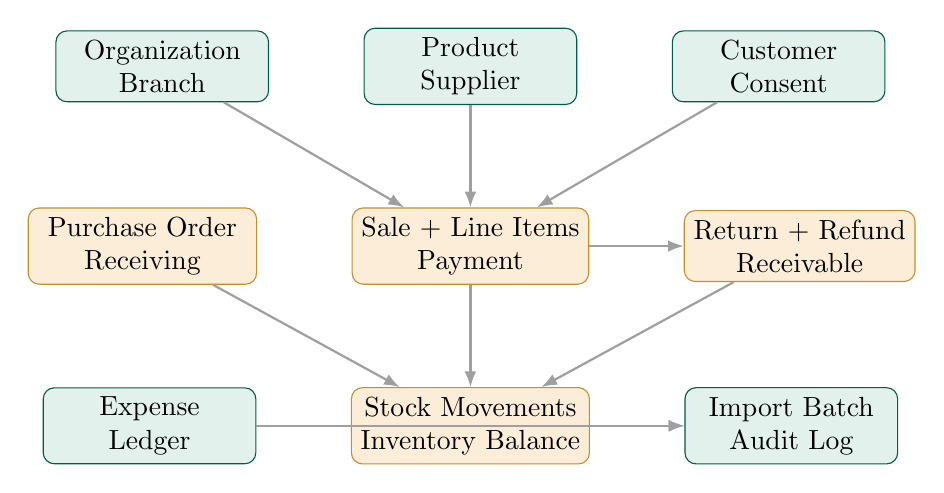
\begin{tikzpicture}[
  entity/.style={draw=dugreen,rounded corners,fill=softgreen,minimum width=2.7cm,minimum height=0.9cm,align=center},
  event/.style={draw=dugold,rounded corners,fill=softorange,minimum width=2.9cm,minimum height=0.9cm,align=center},
  arrow/.style={-{Latex[length=2mm]},thick,draw=gray!75}
]
\node[entity] (org) {Organization\\Branch};
\node[entity,right=1.2cm of org] (product) {Product\\Supplier};
\node[entity,right=1.2cm of product] (customer) {Customer\\Consent};
\node[event,below=1.3cm of product] (sale) {Sale + Line Items\\Payment};
\node[event,left=1.2cm of sale] (purchase) {Purchase Order\\Receiving};
\node[event,right=1.2cm of sale] (return) {Return + Refund\\Receivable};
\node[event,below=1.3cm of sale] (stock) {Stock Movements\\Inventory Balance};
\node[entity,left=1.2cm of stock] (finance) {Expense\\Ledger};
\node[entity,right=1.2cm of stock] (audit) {Import Batch\\Audit Log};
\draw[arrow] (org) -- (sale);
\draw[arrow] (product) -- (sale);
\draw[arrow] (customer) -- (sale);
\draw[arrow] (purchase) -- (stock);
\draw[arrow] (sale) -- (stock);
\draw[arrow] (return) -- (stock);
\draw[arrow] (sale) -- (return);
\draw[arrow] (finance) -- (audit);
\draw[arrow] (stock) -- (audit);
\end{tikzpicture}}
\caption{Proposed canonical operational data model.}
\label{fig:data_model}
\end{figure}

Validation will test uniqueness of business-scoped identifiers, chronological
consistency, nonnegative physical quantities where appropriate, payment/order
reconciliation, cancellation handling and stock-movement balance. Corrections
will be recorded as transformations rather than silently overwriting the source.

\section{Formal Problem Formulation}

For business $b$, branch $l$, product $p$, customer $c$ and time $t$, let

\begin{equation}
  D_t=\{\text{Sales, Stock, Purchases, Expenses, Customers, Payments, Context}\}_{\leq t}.
\end{equation}

\subsection{Performance Evaluation}

For each KPI $K$, the system returns $K(D_t;w,g)$, where $w$ is the reporting
window and $g$ is the aggregation level. Each value retains numerator,
denominator, filters and data-quality status so that the owner can reproduce it.

\subsection{Demand Prediction}

\begin{equation}
\hat{y}_{b,l,p,t+h}=f\!\left(X^{\mathrm{history}}_{t},X^{\mathrm{price}}_{t},
X^{\mathrm{promotion}}_{t},X^{\mathrm{calendar}}_{t:t+h},
X^{\mathrm{market}}_{t}\right),
\label{eq:demand}
\end{equation}
where $\hat{y}$ is expected demand at horizon $h$. Quantile forecasts or
calibrated residual intervals will represent uncertainty. When product-level
forecasts are aggregated, reconciliation will be considered so SKU, category,
branch and business totals remain coherent \cite{hyndman2011hierarchical}.

\subsection{Future Customer Inactivity}

\begin{equation}
q_{c,t}=P\!\left(\text{no purchase in }(t,t+H]\mid X_{c,t}\right),
\label{eq:churn}
\end{equation}
where $X_{c,t}$ contains only records available by cutoff $t$. Horizon $H$ will
be fixed from business purchase cycles before final evaluation.

\subsection{Strategy Optimization}

For an eligible action $a\in A_t$,

\begin{equation}
U(a\mid D_t)=E[\Delta\mathrm{Profit}(a)]-\mathrm{ActionCost}(a)
-\lambda\,\mathrm{Risk}(a),
\label{eq:utility}
\end{equation}
subject to budget, storage, minimum order quantity, supplier lead time,
current/incoming stock and contact consent. This is a transparent operational
objective inspired by the predictive-to-prescriptive transition
\cite{bertsimas2020prescriptive}; its terms will be estimated and sensitivity
tested rather than presented as known constants.

\section{Preprocessing and Historical Snapshots}

The processing order is fixed: validate source and schema; remove or mark exact
duplicates; resolve cancellations and returns; construct the split; fit
imputation, encoding and scaling on training data; build features; train; and
evaluate once on the untouched test. The order prevents statistics from future
periods entering training \cite{kaufman2012leakage}.

Demand features may include lags, rolling location and variability, day of week,
month, festival distance, price, discount, known promotion, stock-out indicator
and external market context. Zero demand caused by no sale is distinguished,
when possible, from zero observed sales caused by no stock. Intermittency will
be measured before choosing temporal granularity and candidate methods.

Customer snapshots will include RFM, tenure, order-value statistics, category
breadth, purchase interval, discount behavior and pre-cutoff return rate. The
label window follows the observation window, with a purge interval when feature
construction or delayed events could overlap it. No customer identifier appears
on both sides of an entity-generalization test.

\section{Candidate Methods and Selection Rules}

Method selection follows a baseline ladder, and eligibility depends on evidence
volume and task structure.

\begin{itemize}
  \item \textbf{Performance:} auditable KPI definitions and rule-based anomaly
  flags establish the descriptive baseline.
  \item \textbf{Demand:} last-value, seasonal-naive, moving-average or
  exponential-smoothing baselines precede ARIMA/SARIMA, Croston-family methods,
  gradient-boosted lag models and, only with adequate sequences, LSTM. Croston
  and the Syntetos--Boylan correction address intermittent demand
  \cite{croston1972intermittent,syntetos2005intermittent}.
  \item \textbf{Inactivity:} a recency or base-rate rule is compared with
  Logistic Regression, Random Forest \cite{breiman2001rf} and XGBoost
  \cite{chen2016xgboost}. Class weighting and decision threshold are selected on
  development data.
  \item \textbf{Segmentation:} scaled RFM features are studied with K-Means.
  Candidate $K$ values are judged by inertia, silhouette, resampling stability
  and business interpretability.
  \item \textbf{Explanation:} coefficient/rule explanations are preferred for
  simple models; SHAP supplies model-behavior attributions for tree models
  \cite{lundberg2017shap,lundberg2020trees}. Displayed reasons will remain
  selective and contextual \cite{miller2019explanation}.
\end{itemize}

A complex candidate will be rejected when it lacks sufficient training history,
cannot beat the relevant baseline on development data, produces unstable
probabilities, or adds operational cost without material value. This rule keeps
the proposed system useful when the scientifically honest answer is a simple
forecast or business rule.

\section{The \system{} Sequential Procedure}

\begin{algorithm}[H]
\caption{\system{} Strategy Recommendation}
\label{alg:bsmart}
\KwIn{Data available at cutoff $D_t$, horizon $H$, constraints $C_t$, validated model/baseline versions $M$, candidate actions $A$}
\KwOut{Ranked feasible recommendations $R_t$}
Verify source, schema, timestamps and organization ownership\;
Create the historical feature snapshot $X_t$\;
Apply transformations fitted on the appropriate training evidence\;
Estimate demand with uncertainty and customer inactivity probabilities\;
Calculate reproducible KPIs and data-quality warnings\;
Generate candidate actions with source and decision-time metadata\;
\ForEach{$a\in A$}{
  Check feasibility under $C_t$\;
  Estimate benefit, cost and uncertainty using declared assumptions\;
  $U(a)\leftarrow E[\Delta\mathrm{Profit}(a)]-\mathrm{Cost}(a)-\lambda\mathrm{Risk}(a)$\;
}
Remove infeasible actions and rank the remainder by $U(a)$\;
Attach concise explanation, uncertainty, cutoff and evidence source\;
Return top-$K$ actions; record owner response and later observable outcome\;
\end{algorithm}

For $N$ invoice lines, $d$ validated fields and $P$ candidate actions, source
validation and feature aggregation are approximately $O(Nd)$ and action ranking
is $O(P\log P)$. Training complexity depends on the selected model and is
measured empirically. Serving reuses versioned artifacts; it must not retrain in
the request path.

\section{Proposed Architecture and Information Flow}

\begin{figure}[H]
\centering
\resizebox{0.98\textwidth}{!}{%
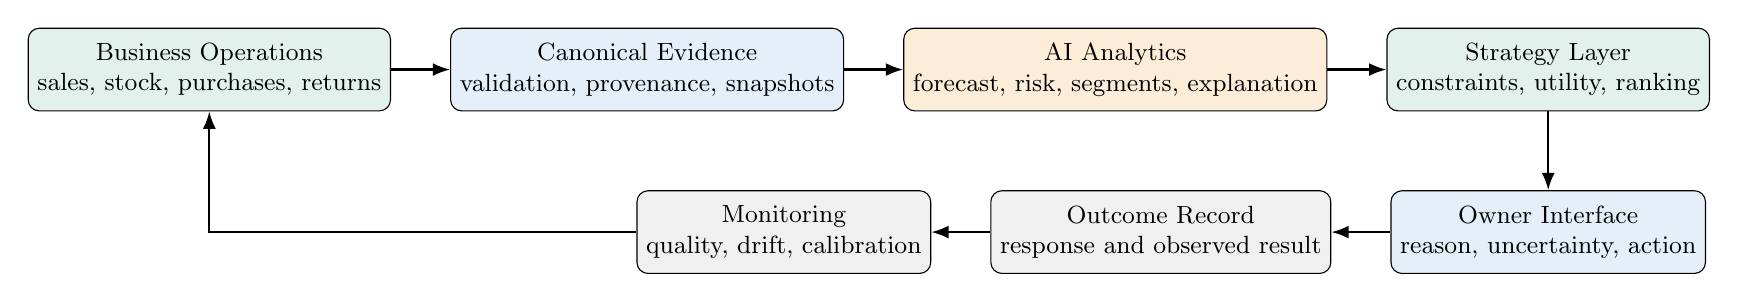
\begin{tikzpicture}[
  block/.style={draw,rounded corners,minimum width=3.0cm,minimum height=1.05cm,align=center,font=\small},
  arrow/.style={-{Latex[length=2.2mm]},thick},node distance=0.75cm
]
\node[block,fill=softgreen] (ops) {Business Operations\\sales, stock, purchases, returns};
\node[block,fill=softblue,right=of ops] (canon) {Canonical Evidence\\validation, provenance, snapshots};
\node[block,fill=softorange,right=of canon] (ai) {AI Analytics\\forecast, risk, segments, explanation};
\node[block,fill=softgreen,right=of ai] (strategy) {Strategy Layer\\constraints, utility, ranking};
\node[block,fill=softblue,below=1.0cm of strategy] (ui) {Owner Interface\\reason, uncertainty, action};
\node[block,fill=softgray,left=of ui] (outcome) {Outcome Record\\response and observed result};
\node[block,fill=softgray,left=of outcome] (monitor) {Monitoring\\quality, drift, calibration};
\draw[arrow] (ops) -- (canon);
\draw[arrow] (canon) -- (ai);
\draw[arrow] (ai) -- (strategy);
\draw[arrow] (strategy) -- (ui);
\draw[arrow] (ui) -- (outcome);
\draw[arrow] (outcome) -- (monitor);
\draw[arrow] (monitor.west) -| ($(ops.south)+(0,-0.15)$) -- (ops.south);
\end{tikzpicture}}
\caption{Proposed \system{} architecture and accountable feedback loop.}
\label{fig:bsmart_architecture}
\end{figure}

The information flow is intentionally one-directional at prediction time:
future outcomes cannot alter the snapshot that produced an earlier result.
Outcomes enter later through the monitoring path and become eligible training
evidence only in a new, versioned cycle. This separation makes it possible to
reproduce what the system knew when an action was proposed.

\section{Evaluation Protocol}

\subsection{Forecasting Evaluation}

All forecasting splits preserve time. Candidate methods are selected through
rolling-origin or expanding-window validation, followed by one evaluation on a
final untouched period. For actual values $y_i$ and forecasts $\hat y_i$,

\begin{align}
\mathrm{MAE} &= \frac{1}{n}\sum_{i=1}^{n}|y_i-\hat y_i|,\\
\mathrm{RMSE} &= \sqrt{\frac{1}{n}\sum_{i=1}^{n}(y_i-\hat y_i)^2},\\
\mathrm{WAPE} &= \frac{\sum_i|y_i-\hat y_i|}{\sum_i|y_i|}.
\end{align}

MASE will support comparison across scales and avoid some defects of percentage
errors \cite{hyndman2006accuracy}. Prediction-interval coverage and width or a
proper scoring rule will evaluate uncertainty \cite{gneiting2007scoring}.
Results will be stratified by demand volume and intermittency rather than hiding
failure on low-volume items in one aggregate.

\subsection{Customer and Segmentation Evaluation}

Inactivity models will report outcome prevalence, PR-AUC, ROC-AUC, Lift@10\%,
Brier score and reliability plots. The emphasis on PR measures follows their
value under imbalance \cite{saito2015pr}; calibration is assessed separately
because a useful ranking can still produce misleading probabilities
\cite{niculescu2005calibration}. Thresholds and contact fractions are chosen on
validation evidence using declared costs, not adjusted after viewing the test.

Clustering evaluation will report inertia, silhouette, cluster stability,
minimum cluster size and RFM profiles. The final interpretation will be reviewed
with domain participants. A low-separation result will be reported as such; the
existence of clusters will not be treated as proof of natural customer types.

\subsection{Ablation, Robustness and Statistical Analysis}

Planned ablations remove one feature family at a time: local calendar,
price/promotion, market context and customer-history extensions. Additional
comparisons examine global versus business-specific models and real-only versus
clearly controlled augmentation. All paired comparisons use the same test
instances or forecast origins.

Uncertainty will be summarized with paired block bootstrap intervals across
time or business units, as appropriate. Model differences will be reported with
effect size and interval, not only a significance label. Sensitivity analysis
will vary lead time, shortage cost, holding cost, action cost and risk penalty in
Equation~\ref{eq:utility}.

\subsection{Decision, Usability and Scalability Evaluation}

Replenishment policies will face identical observed or replayed demand paths.
The comparison records stock-out units, average inventory, holding cost,
shortage cost and total cost. Retention ranking will use expected value only
when response benefit, contact cost and consent are available; otherwise it will
remain a prioritization study, not a profit claim \cite{verbeke2012profit}.

Owner evaluation will use realistic tasks in a counterbalanced within-subject
design when the sample permits. Measures include task correctness, completion
time, error count, confidence and perceived usability. Participants may explain
their decision in their own words, allowing the study to detect plausible but
misunderstood explanations.

Scalability tests will use generated data only and will remain separate from
accuracy results. Planned sizes are 100, 500, 1,000, 10,000, 100,000 and
1,000,000 transaction lines. Measures include import and preprocessing time,
training time, prediction latency, API throughput, peak memory, artifact size
and representative query latency. Any association-rule support experiment will
be reported only after the corresponding algorithm exists and has been run.

\subsection{Monitoring Plan}

Monitoring will distinguish schema or data-quality failure, input shift,
calibration change and outcome-performance change. Alerts will not automatically
authorize retraining. A new model must repeat the validation protocol and retain
its training window, features, parameters and comparison result. This follows
the concept-drift literature's emphasis on both adaptation and appropriate
evaluation \cite{gama2014drift}.

\section{Threats to Validity and Planned Controls}

\begin{table}[H]
\centering
\small
\caption{Principal validity threats and planned controls.}
\label{tab:validity_controls}
\begin{tabularx}{\textwidth}{p{0.22\textwidth}p{0.30\textwidth}Y}
\toprule
\textbf{Threat} & \textbf{How it may distort evidence} & \textbf{Planned control} \\
\midrule
Selection bias & Cooperative firms may be more digitally mature & Describe recruitment and firms; restrict generalization \\
Leakage & Future or target-derived data inflate performance & Availability table, cutoff snapshots, grouped/temporal split \\
Stock-out censoring & Observed sales understate unconstrained demand & Retain stock state; stratify or flag censored periods \\
Small/short series & Complex models overfit & Eligibility rule, simple baselines, rolling validation \\
Dataset mismatch & Foreign/public tasks are mistaken for local evidence & Evidence tiers and separate result tables \\
Uncertain costs & Utility ranking depends on weak assumptions & Owner-validated ranges and sensitivity analysis \\
Novelty/learning effect & Interface condition benefits from presentation order & Counterbalance tasks and collect task-level timing \\
Concept drift & Festival, price or behavior relations change & Time-based tests and post-deployment monitoring plan \\
\bottomrule
\end{tabularx}
\end{table}

\section{Two-Semester Work Plan}

The project period is February 2026--February 2027. The first semester defines
the problem, evidence base and proposed artifact; the second emphasizes primary
data, implementation completion, controlled evaluation and consolidation. The
schedule in Table~\ref{tab:gantt} is dependency-aware: the final model study
cannot precede ethics/data readiness, and the final conclusions cannot precede
the frozen evaluation.

\begin{landscape}
\begin{table}[H]
\centering
\scriptsize
\setlength{\tabcolsep}{3.2pt}
\renewcommand{\arraystretch}{1.35}
\caption{Project timeline from February 2026 to February 2027.}
\label{tab:gantt}
\begin{tabular}{p{0.24\linewidth}*{13}{c}}
\toprule
\textbf{Work package} & \rotatebox{90}{Feb 26} & \rotatebox{90}{Mar 26} & \rotatebox{90}{Apr 26} & \rotatebox{90}{May 26} & \rotatebox{90}{Jun 26} & \rotatebox{90}{Jul 26} & \rotatebox{90}{Aug 26} & \rotatebox{90}{Sep 26} & \rotatebox{90}{Oct 26} & \rotatebox{90}{Nov 26} & \rotatebox{90}{Dec 26} & \rotatebox{90}{Jan 27} & \rotatebox{90}{Feb 27} \\
\midrule
WP1: Background study and problem formulation & \cellcolor{softgreen} & \cellcolor{softgreen} & \cellcolor{softgreen} & & & & & & & & & & \\
WP2: Requirements, ethics and data protocol & & & \cellcolor{softgreen} & \cellcolor{softgreen} & \cellcolor{softgreen} & \cellcolor{softgreen} & & & & & & & \\
WP3: Framework, schema and evaluation design & & & & \cellcolor{softgreen} & \cellcolor{softgreen} & \cellcolor{softgreen} & \cellcolor{softgreen} & \cellcolor{softgreen} & & & & & \\
WP4: Core artifact implementation & & & & & & \cellcolor{softblue} & \cellcolor{softblue} & \cellcolor{softblue} & \cellcolor{softblue} & & & & \\
WP5: Partner onboarding and primary data & & & & & & & & \cellcolor{softblue} & \cellcolor{softblue} & \cellcolor{softblue} & & & \\
WP6: Model development and internal validation & & & & & & & & & \cellcolor{softblue} & \cellcolor{softblue} & \cellcolor{softblue} & & \\
WP7: Frozen tests, ablations and scale study & & & & & & & & & & & \cellcolor{softorange} & \cellcolor{softorange} & \\
WP8: Usability and decision-impact study & & & & & & & & & & & & \cellcolor{softorange} & \cellcolor{softorange} \\
WP9: Final writing, audit and defence preparation & & & & & & & & & & & \cellcolor{softorange} & \cellcolor{softorange} & \cellcolor{softorange} \\
\bottomrule
\end{tabular}

\vspace{0.3cm}
\textit{Legend:} \colorbox{softgreen}{Phase-I research foundation}\quad
\colorbox{softblue}{build and data preparation}\quad
\colorbox{softorange}{evaluation and consolidation}.
\end{table}
\end{landscape}

\begin{table}[H]
\centering
\small
\caption{Milestones, exit criteria and contingency.}
\label{tab:milestones}
\begin{tabularx}{\textwidth}{p{0.17\textwidth}p{0.18\textwidth}Y Y}
\toprule
\textbf{Milestone} & \textbf{Target} & \textbf{Exit criterion} & \textbf{Contingency} \\
\midrule
M1: Initial report & September 2026 & Problem, verified background, proposed method and approved plan & Revise scope/RQs before model lock \\
M2: Data readiness & November 2026 & Ethics/agreement complete; manifest and quality report for eligible primary data & Narrow the primary task; retain public data only as external procedure checks \\
M3: Model freeze & December 2026 & Baselines, features, splits, metrics and seeds fixed before final test & Prefer simpler eligible models when volume is inadequate \\
M4: Evaluation freeze & January 2027 & Untouched tests, ablations, intervals, decision and scale analyses complete & Report inconclusive/negative findings; do not retune on test \\
M5: Final thesis & February 2027 & Chapters complete; citations, claims, figures and reproducibility artifacts audited & Remove unsupported claims and document remaining limitations \\
\bottomrule
\end{tabularx}
\end{table}

The critical path runs through ethics and primary-data readiness (M2), model
freeze (M3) and evaluation freeze (M4). Weekly progress review will track a
deliverable, its evidence and its next dependency. Schedule pressure will not be
handled by converting a public or generated-data result into a primary local
claim.

\section{Expected Methodological Outputs}

At completion, the methodology is expected to yield a documented canonical
schema and data dictionary, partner data protocol, versioned feature snapshots,
baseline and candidate model specifications, a constraint-aware recommendation
procedure, a reproducible evaluation package and an owner-study instrument.
Implementation detail, observed numerical results and conclusions will be added
to the reserved chapters only after the corresponding milestones are satisfied.

\cleardoublepage
\chapter{Implementation}
\label{chapter_implementation}

\section{Implementation Status}

As of \reportdate, the repository contains a complete local thesis MVP. It is
not represented as a finished commercial ERP. The operational, analytical and
strategy layers execute locally, and current safeguards distinguish a trained
real-data model from a transparent baseline. External sign-in, public deployment,
fiscal integration, native mobile/offline synchronization and automated campaigns
are intentionally deferred.

\begin{table}[H]
\centering
\small
\caption{Current functional status.}
\label{tab:implementation_status}
\begin{tabularx}{\textwidth}{p{0.24\textwidth}p{0.14\textwidth}Y}
\toprule
\textbf{Component} & \textbf{Status} & \textbf{Implemented boundary} \\
\midrule
Business operations & Complete MVP & Catalogue, branch, customer, supplier, stock, sales, purchase, return, expense and ledgers \\
Data intake & Complete MVP & Durable CSV/XLSX import, validation, checksum/provenance and canonical sales export \\
Research analytics & Complete MVP & Segmentation, forecasting, churn, return, leakage ablation and SHAP artifacts \\
Real-data training & Complete MVP & Chronological demand pipeline and purged future-repeat pipeline \\
Strategy layer & Complete MVP & Constraint-aware reorder and consent-safe retention ranking; baseline/model provenance \\
API and dashboard & Complete MVP & FastAPI routes plus React research and Bangla-first operational pages \\
Automated verification & Passing & Six backend tests pass; production frontend builds \\
Primary SME validation & Pending & Consenting Bangladeshi invoice/stock data and field evaluation required \\
Association-rule module & Not implemented & Minimum-support scalability experiment remains out of current results \\
Public production deployment & Deferred & OAuth, managed database, monitoring, billing and hardware integration outside current MVP \\
\bottomrule
\end{tabularx}
\end{table}

\section{Technology Stack}

The backend uses Python 3.12, FastAPI, Pydantic, SQLAlchemy and Alembic. SQLite
supports the local prototype, with foreign-key enforcement; the configuration
layer permits a production database later. The analytical stack comprises
pandas, NumPy, SciPy, scikit-learn, XGBoost, statsmodels, TensorFlow, SHAP,
Matplotlib and Seaborn. Models and preprocessing objects are persisted with
pickle, Joblib or the native Keras format as appropriate.

The frontend uses React, React Router, Recharts and Vite. A HashRouter permits
the static production build to be served without server-side route rewriting.
Research views remain technical and English-oriented, while daily operational
views are Bangla-first. The current local database is \texttt{bsmart.db}; schema
migrations are versioned under \texttt{migrations/}.

\section{Repository and Layered Architecture}

The implementation separates domain transactions, analytical service code and
presentation. Table~\ref{tab:code_map} maps major code to its responsibility.

\begin{table}[H]
\centering
\small
\caption{Implementation map.}
\label{tab:code_map}
\begin{tabularx}{\textwidth}{p{0.32\textwidth}Y}
\toprule
\textbf{Module or directory} & \textbf{Responsibility} \\
\midrule
\texttt{api/domain\_models.py} & Multi-tenant operational schema and audit/provenance entities \\
\texttt{api/commerce\_routes.py} & Products, inventory adjustments and atomic sales \\
\texttt{api/finance\_routes.py} & Purchases, receiving, payments, returns, refunds, expenses and ledgers \\
\texttt{api/directory\_routes.py} & Branches, staff, customers and suppliers \\
\path{api/data_import_routes.py} & Durable imports, validation, canonical export and model-training trigger \\
\texttt{api/analytics\_routes.py} & Tenant-scoped KPI and constraint-aware recommendations \\
\texttt{predict.py} & Loads fixed research artifacts and provides inference/service functions \\
\texttt{upload\_service.py} & Anonymous dataset mapping, analysis and dataset-specific future-repeat training \\
\texttt{ml/real\_pipeline.py} & Chronological real-data demand and future-repeat training \\
\texttt{ml/serving.py} & Loads organization-specific demand artifacts for strategy recommendations \\
\texttt{ml/market\_prices.py} & Bangladesh commodity-price benchmarks and market-context table \\
\path{ml/real_data_validation.py} & UCI and Bangladeshi public-real method validation \\
\texttt{frontend/src/pages/} & Operational and research-mode application screens \\
\texttt{tests/} & Authentication, tenant/database, commerce and analytics invariants \\
\bottomrule
\end{tabularx}
\end{table}

\begin{figure}[H]
\centering
\resizebox{0.98\textwidth}{!}{%
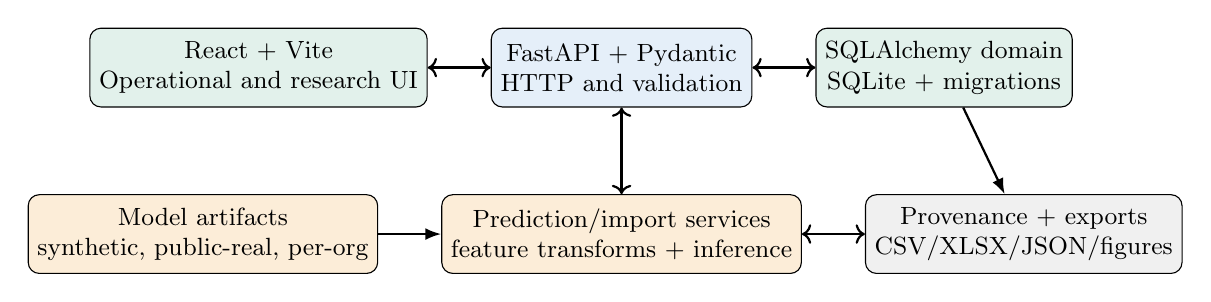
\begin{tikzpicture}[
  box/.style={draw,rounded corners,minimum height=1cm,minimum width=3.2cm,align=center,font=\small},
  arrow/.style={-{Latex[length=2mm]},thick},node distance=0.8cm
]
\node[box,fill=softgreen] (react) {React + Vite\\Operational and research UI};
\node[box,fill=softblue,right=of react] (api) {FastAPI + Pydantic\\HTTP and validation};
\node[box,fill=softgreen,right=of api] (domain) {SQLAlchemy domain\\SQLite + migrations};
\node[box,fill=softorange,below=1.1cm of api] (services) {Prediction/import services\\feature transforms + inference};
\node[box,fill=softorange,left=of services] (models) {Model artifacts\\synthetic, public-real, per-org};
\node[box,fill=softgray,right=of services] (files) {Provenance + exports\\CSV/XLSX/JSON/figures};
\draw[arrow,<->] (react)--(api);
\draw[arrow,<->] (api)--(domain);
\draw[arrow,<->] (api)--(services);
\draw[arrow] (models)--(services);
\draw[arrow,<->] (services)--(files);
\draw[arrow] (domain)--(files);
\end{tikzpicture}}
\caption{Implemented local application architecture.}
\label{fig:implemented_architecture}
\end{figure}

\section{Operational Layer}

\subsection{Tenant and Branch Isolation}

An organization contains branches and memberships. Domain rows carry an
organization identifier, and request dependencies resolve the active membership
before a query or mutation. Duplicate SKUs are rejected within one tenant while
separate tenants may use the same SKU text. The current authentication layer
supports local prototype identity and optional JWT verification; Google or other
external OAuth is not implemented.

\subsection{Catalogue, Inventory and Sales}

A product stores SKU, category, unit, cost, selling price, barcode and reorder
level. Inventory adjustment creates an append-only stock movement and updates the
materialized balance. Sale creation validates stock and records the order, line
items, payments and stock decrements within one database transaction. Supported
settlement methods include cash, bKash, Nagad, Bangla QR, card and due sales.

\subsection{Purchasing, Returns and Accounts}

Purchase orders support partial or full receiving; received lines update stock
and supplier payable state. A sale return can optionally restock goods and can
create a refund or receivable adjustment. Expenses and payable/receivable ledger
entries feed a 30-day operational dashboard. These flows create the data needed
for future demand and business-impact evaluation instead of requiring an
unrelated research spreadsheet.

\section{Durable Data Intake}

The anonymous research upload flow parses CSV/XLSX columns, suggests mappings,
cleans transactions and provides overview, forecast, segmentation, product and
future-repeat analysis. The operational import flow is durable: it writes the
source file, checksum, row count and validation status to an ImportBatch record.
The canonical export provides the exact schema expected by the real-data training
pipeline.

Import validation checks tenant, branch, invoice, line, SKU and timestamp keys;
monetary identities; return/cancellation treatment; missingness; and cross-tenant
collisions. Phone data are hashed for the operational customer directory and are
not included in research features.

\section{Analytical Pipeline}

The original numbered research scripts form a reproducible sequence:

\begin{enumerate}[label=\texttt{\arabic*.},start=0]
  \item \texttt{00\_normalize\_dataset.py}: convert the flat synthetic CSV to
  six dimensions and one transaction fact, then create a verified merge.
  \item \texttt{01\_preprocessing.py} and \texttt{01b\_customer\_features.py}:
  clean, encode, engineer RFM/calendar features and create leakage-safe customer
  splits.
  \item \texttt{02\_classification.py} and
  \texttt{02b\_classification\_v2.py}: retain the legacy result for ablation and
  train the honest customer-level XGBoost, Random Forest and Logistic Regression
  comparison.
  \item \texttt{03\_clustering.py}: evaluate candidate $K$ values and fit
  K-Means on RFM profiles.
  \item \texttt{04\_forecasting.py}: compare LSTM, ARIMA(2,1,2) and a
  seasonal-naive forecast on the same holdout.
  \item \texttt{05\_shap\_analysis.py}: generate global/local SHAP artifacts;
  current legacy plots are interpreted as a leakage audit where relevant.
  \item \texttt{06\_final\_report.py}: aggregate metrics and figures.
  \item \path{07_return_prediction.py} and
  \path{08_churn_prediction.py}: evaluate pre-dispatch return and future
  inactivity risk using imbalance-aware metrics.
\end{enumerate}

The separate real-data path uses chronological splits and organization-specific
artifacts. A trained demand model is stored at
\begin{center}
\path{artifacts/real/<organization-id>/demand_model.joblib}.
\end{center}
Serving first looks for this artifact; when it does not exist or lacks history
for a SKU, a clearly labelled 28-day demand-rate baseline is used.

\section{Strategy Optimization Layer}

The recommendation endpoint reads only the active tenant's canonical records.
For each product it combines observed or modelled demand rate, current stock,
reorder level and lead time to generate a candidate reorder. For customers it
uses recency/value information and contact consent to generate retention
candidates. The action includes estimated utility, reason, method and a
\texttt{confidence} field with value \texttt{model} or \texttt{baseline}.

This provenance is a scientific and user-interface control. The UI does not
rename a heuristic as AI while data are insufficient. Automated campaigning is
not performed; the system ranks consented customers for human review.

\section{API and User Interface}

The API exposes health, research dashboard, customer, prediction, anonymous
upload, operational commerce, directory, finance, data import, training and
strategy routes. The React application contains the following page groups:

\begin{itemize}
  \item \textbf{Daily operations:} setup, sales, products, inventory, purchases,
  returns, directory, accounts and the 30-day operational dashboard.
  \item \textbf{Strategy:} constraint-aware action cards with method/confidence.
  \item \textbf{Research mode:} overview, dataset upload, what-if analysis,
  segments, customers, forecast, model report and real-data validation.
\end{itemize}

The current design keeps evaluator-facing model detail in English and
owner-facing daily tasks in Bangla. A final usability study will test whether
this split and the explanation cards improve decisions.

\section{Verification and Build Status}

On \reportdate, \texttt{python -m pytest -q} completes successfully with six
passing tests. The tests cover token behavior, wrong-audience rejection,
tenant-scoped SKU/stock invariants, duplicate-SKU rejection, atomic sale/stock
decrement and operational analytics. The set is a high-value smoke suite rather
than complete coverage; failure-path, concurrency, migration and browser tests
remain to be expanded.

The command \texttt{npm run build} transforms 611 modules and completes the
production build successfully. The main minified JavaScript asset is about
769.61 kB (219.15 kB gzip), triggering a chunk-size warning. Route-level dynamic
imports and code splitting are therefore an implementation task before public
deployment, but the warning does not prevent the local thesis demonstration.

\section{Reproducibility}

The Python 3.12 environment is used because TensorFlow support is not available
for the system's newer default interpreter. Random seeds are set where supported,
but minor LSTM variation remains possible because early stopping and backend
operations are not fully deterministic. Deterministic baseline results and stored
artifacts preserve the ranking. The repository build guide lists the
commands and output map.

\cleardoublepage
\chapter{Experimental Results}
\label{chapter_experimentalResults}

% This chapter is intentionally reserved until the proposed experiments are run.

\cleardoublepage
\chapter{Conclusions}
\label{chapter_conclusion}

\section{Current-Stage Conclusion}

This initial report establishes a focused foundation for an AI-powered business
analytics system for Bangladeshi retail SMEs. The central problem is not merely
the absence of prediction models. It is the missing, trustworthy connection
between operational records, temporally valid analytics and a feasible owner
decision. A forecast has limited practical value if its source cannot be traced,
its test contains future information, or the result ignores cash, stock and lead
time. A customer-risk score is similarly incomplete when its probability is
uncalibrated or the proposed contact does not respect consent.

The evidence leads to four conclusions. Bangladesh-specific studies make
workflow fit, perceived value, cost and local technology use necessary design
considerations \cite{hoque2016ict,shahadat2023digital,hazra2021mfs}. Retail and
inventory research requires explicit treatment of intermittency, hierarchy,
forecast error and stock consequences
\cite{fildes2022retail,syntetos2005intermittent,hyndman2011hierarchical,
syntetos2010stock}. Leakage control, imbalance-aware evaluation, probability
calibration and understandable evidence are scientific safeguards
\cite{kaufman2012leakage,saito2015pr,niculescu2005calibration,lundberg2017shap}.
The resulting research gap is integrative: these principles have not yet been
evaluated together in a bounded Bangladesh-oriented SME workflow.

The proposed \system{} framework responds through a traceable sequence of
operational events, canonical evidence, historical snapshots, baseline/model
comparison, uncertainty and explanation, constraint-aware action ranking,
owner response and later outcome monitoring. Its proposed contribution is this
governed sequence and its evaluation, not the invention of a new classifier or
an unsupported claim that a complex model will always perform best.

The report therefore supplies a testable path into the next phase: ethics and
partner-data readiness, model freeze, untouched evaluation, usability tasks and
decision-impact analysis. It does not yet establish system effectiveness. Final
claims must follow the observed evidence, including any result in which a simple
baseline wins, explanations show no measurable advantage, or the available data
cannot support a research question.

\cleardoublepage

\addtocontents{toc}{\vspace{1em}}
\backmatter
\label{Bibliography}
\lhead{\emph{Bibliography}}
\bibliographystyle{acm}
\bibliography{Bibliography}

\end{document}
